% @author Marcel Ruland (2018)
% !TEX encoding = UTF-8 Unicode
% !TEX TS-program = LuaLaTeX
\documentclass[aspectratio=169]{beamer}
%\setbeameroption{show notes}


%*******************Beamer Theme*******************
\usetheme{Dresden}				% use Dresden theme
\useinnertheme{rectangles}		% rectangles for itemize environment etc
\useoutertheme{infolines}		% lots of info using little space
\setbeamercovered{transparent}	% set covered items to 85% alpha
%**************************************************

%******************Packages in Use*****************
\usepackage[english]{babel}						% English language support
\usepackage{ttjenevers}							% use TT Jenevers for rm
\usepackage{ttcommons}							% use TT Commons for sf
\setmonofont[Scale=MatchLowercase]{Envy Code R}	% use Envy Code R for tt
\usepackage{microtype}							% improved typography
\usepackage{natbib}								% bibliography
\bibliographystyle{newharvard}					% custom Harvard bibliography style
\usepackage{tabularx}							% more spacing options for tables
\usepackage{array}								% >{} syntax for table formatting
\usepackage{url}								% typeset urls
\usepackage{tikz}								% TikZ ist kein Zeichenprogramm
\usetikzlibrary{positioning}					% relative positioning of nodes
\usetikzlibrary{arrows}							% more arrows
\usetikzlibrary{calc}							% calculations
\usepackage{pgfplots}							% plotting functions
\pgfplotsset{compat=1.15}
%**************************************************

%*******************New Commands*******************
\newcommand{\code}[1]{\texttt{#1}}
\newcommand{\sfmath}[1]{\(\mathsf{#1}\)}		% inline sf maths
\newcommand{\fpmlabel}[1]{\(\mathcal{#1}\)}		% typeset label

\newcommand{\shorttitle}{Applying \textsc{fpm} to Multimodal Behaviour in Interaction}
\newcommand{\longtitle}{Applying Frequent Pattern Mining to \\ Multimodal Behaviour in Interaction}
\newcommand{\shortauthor}{K.~Rohlfing, {\addfontfeature{Style=Alternate}M.~Ruland}, S.~Henzgen}
%**************************************************

%****************** New Colours *******************
%\definecolor{graphgreen}{cmyk}{0.76,0.25,0.8,0.18}
%\definecolor{graphred}{cmyk}{0.01,0.92,0.86,0.14}
\definecolor{alert}{HTML}{FF0400}
\definecolor{beamerblue}{HTML}{3333B2}
%**************************************************


\title[\shorttitle]{\longtitle}
%\subtitle{Visualising Significant Patterns}
\institute{Paderborn University}
\author[\shortauthor]{Katharina Rohlfing \and {\addfontfeature{Style=Alternate}Marcel Ruland} \and Sascha Henzgen}
\date[6/6/2018]{July 6, 2018}

\begin{document}

\frame{\titlepage}


\section{Preliminaries}%%%%
\frame{
	\frametitle{Basic Concepts}
	\begin{columns}
		\column{0.35\textwidth}
		\begin{itemize}
			\item turn
			\item turn-taking
			\item uni- vs multimodality
		\end{itemize}
		\column{0.65\textwidth}
		\begin{figure}
			\includegraphics[width=\textwidth]{../aux/img/dummy_basic_concepts.png}
			\caption{Responses in conversation are fast\textsuperscript{[1]}}
		\end{figure}
	\end{columns}
	
	\vfill
	
	{\tiny\textsuperscript{[1]}\textsc{Levinson}, Stephen C.\ (2016): ``Turn-taking in human communication: Origins and implications for language processing.'' \textit{Trends in Cognitive Sciences} \textbf{20} (1): 6--14}
}
\frame{
	\frametitle{Turn-Taking -- Why do we care?}
	\begin{columns}
		\column{0.35\textwidth}
		\begin{itemize}
			\item language universal
			\item present in related species
			\item present in early infancy
		\end{itemize}
		\column{0.65\textwidth}
		\begin{figure}
			% !TEX root = ../../beamer/ba_beamer_master.tex
% @author Marcel Ruland (2018)
\newcommand{\apewidth}{1.5cm}

\begin{tikzpicture}[
	every node/.append style={inner sep=0cm,align=center,text width=\apewidth,font=\tiny},
	node distance=0.1cm and 0.1cm,
]

%% top pics
\node							(lepilemur)		{\includegraphics[width=\apewidth]{../aux/img/species/lepilemur.jpg}};
\node[right=of lepilemur]		(callithrix)	{\includegraphics[width=\apewidth]{../aux/img/species/callithrix.jpg}};
\node[right=of callithrix]		(cebuella)		{\includegraphics[width=\apewidth]{../aux/img/species/cebuella.jpg}};
\node[right=of cebuella]		(callicebus)	{\includegraphics[width=\apewidth]{../aux/img/species/callicebus.jpg}};
\node[right=of callicebus]		(saimiri)		{\includegraphics[width=\apewidth]{../aux/img/species/saimiri.jpg}};
\node[right=of saimiri]			(cercopithecus)	{\includegraphics[width=\apewidth]{../aux/img/species/cercopithecus.png}};

%% bottom apes
\node[below=1.5cm of lepilemur]	(hylobates)		{\includegraphics[width=\apewidth]{../aux/img/species/hylobates.jpg}};
\node[right=of hylobates]		(orangutans)	{\includegraphics[width=\apewidth]{../aux/img/species/orangutans.jpg}};
\node[right=of orangutans]		(gorillas)		{\includegraphics[width=\apewidth]{../aux/img/species/gorillas.jpg}};
\node[right=of gorillas]		(chimpanzees)	{\includegraphics[width=\apewidth]{../aux/img/species/chimpanzees.png}};
\node[right=of chimpanzees]		(humans)		{\includegraphics[width=\apewidth]{../aux/img/species/humans.jpg}};
\node[right=of humans]			(diaemus)		{\includegraphics[width=\apewidth]{../aux/img/species/diaemus.jpg}};

%% braces
% prosimians
\draw[decorate,decoration={brace,amplitude=5pt}]
(lepilemur.north west) -- (lepilemur.north east)
node[midway,yshift=0.35cm]{\scriptsize{prosimians}};

% monkeys
\draw[decorate,decoration={brace,amplitude=5pt}]
(callithrix.north west) -- (cercopithecus.north east)
node[midway,yshift=0.35cm]{\scriptsize{monkeys}};

% apes
\draw[decorate,decoration={brace,amplitude=5pt}]
(humans.south east) -- (hylobates.south west)
node[midway,yshift=-0.35cm]{\scriptsize{apes}};

% bats
\draw[decorate,decoration={brace,amplitude=5pt}]
(diaemus.south east) -- (diaemus.south west)
node[midway,yshift=-0.35cm]{\scriptsize{bats}};

%% top labels
\node[below=of lepilemur]		{lepilemur edwardsi};
\node[below=of callithrix]		{callithrix jacchus};
\node[below=of cebuella]		{cebuella pygmaea};
\node[below=of callicebus]		{callicebus cupreus};
\node[below=of saimiri]			{saimiri};
\node[below=of cercopithecus]	{cercopithecus campbelli};

%% bottom labels
\node[above=of hylobates]		{hylobates syndactylus};
\node[above=of orangutans]		{orangutans};
\node[above=of gorillas]		{gorillas};
\node[above=of chimpanzees]		{chimpanzees};
\node[above=of humans]			{humans};
\node[above=of diaemus]			{diaemus youngi};
\end{tikzpicture}
			\caption{Turn-taking across species}
		\end{figure}
	\end{columns}
}


\section{Method}%%%%
\frame{
	\frametitle{Video Material}
	\begin{figure}
		\center
		\includegraphics[width=\textwidth]{../aux/img/video_vp_08_compact.png}
		\caption{Example of recorded material}
	\end{figure}
}
\frame{
	\frametitle{Annotating the Videos}
	\only<+>{
		\begin{figure}
			\center
			\includegraphics[width=\textwidth]{../aux/img/elan.png}
			\caption{\textsc{elan} screenshot}
		\end{figure}
	}
	\only<+>{
		\begin{columns}
			\column{0.5\textwidth}
			\begin{itemize}
				\item intervals
				\item intervals from different modalities
				\item modalities from different sources
			\end{itemize}
			\column{0.5\textwidth}
			\begin{figure}
				\center
				\includegraphics[width=\textwidth]{../aux/img/elan_cropped.png}
				\caption{\textsc{elan} screenshot}
			\end{figure}
		\end{columns}
	}
}
\frame{
	\frametitle{What counts as a rule?}
	\begin{columns}
		\column{0.4\textwidth}
		\begin{enumerate}
			\item[]\fpmlabel{A} \rightarrow \fpmlabel{B} represents one of two cases:\textsuperscript{[1]}
			\item interval of \fpmlabel{A} starts before interval of \fpmlabel{B} \textbf{or}
			\item interval of \fpmlabel{A} and \fpmlabel{B} start at the same time
			\item[]~
			\item[]\textbf{and} \fpmlabel{B} begins before \fpmlabel{A} ends
		\end{enumerate}
		\column{0.6\textwidth}
		\begin{figure}
			% !TEX root = ../../beamer/ba_beamer_master.tex
% @author Marcel Ruland (2018)
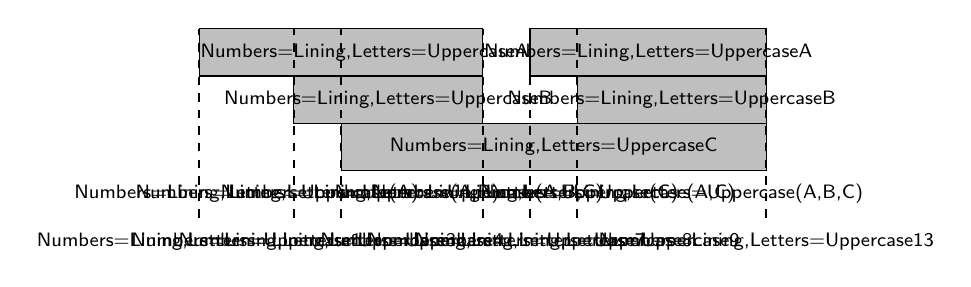
\begin{tikzpicture}[
	scale=0.6,
	every node/.append style={font=\scriptsize\sffamily\addfontfeature{Numbers=Lining,Letters=Uppercase}}]
	% boxes
	\draw [fill=lightgray] (0,4) rectangle (6,5);  % A1
	\node at (3.5,4.5) {A};
	
	\draw [fill=lightgray] (7,4) rectangle (12,5);  % A2
	\node at (9.5,4.5) {A};
	
	\draw [fill=lightgray] (2,3) rectangle (6,4);  % B1
	\node at (4,3.5) {B};
	
	\draw [fill=lightgray] (8,3) rectangle (12,4);  % B2
	\node at (10,3.5) {B};
	
	\draw [fill=lightgray] (3,2) rectangle (12,3);  % C
	\node at (7.5,2.5) {C};
	
	% item sets
	\node at (1,1.5) {(A)};
	\node at (2.5,1.5) {(A,B)};
	\node at (4.5,1.5) {(A,B,C)};
	\node at (6.5,1.5) {(C)};
	\node at (7.5,1.5) {(A,C)};
	\node at (10,1.5) {(A,B,C)};
	
	% time points
	\node at (0,0.5) {1};
	\node at (2,0.5) {3};
	\node at (3,0.5) {4};
	\node at (6,0.5) {7};
	\node at (7,0.5) {8};
	\node at (8,0.5) {9};
	\node at (12,0.5) {13};
	
	% time point lines
	\draw [dashed, thick] (0,1) -- (0,5);
	\draw [dashed, thick] (2,1) -- (2,5);
	\draw [dashed, thick] (3,1) -- (3,5);
	\draw [dashed, thick] (6,1) -- (6,5);
	\draw [dashed, thick] (7,1) -- (7,5);
	\draw [dashed, thick] (8,1) -- (8,5);
	\draw [dashed, thick] (12,1) -- (12,5);
\end{tikzpicture}
		\end{figure}
	\end{columns}
	
	\vfill
	
	{\tiny\textsuperscript{[1]}\textsc{Rohlfing}, Katharina; \textsc{Leonardi}, Giuseppe; \textsc{Hüllermeier}, Eyke; \textsc{Raczaszek-Leonardi}, Johanna; and \textsc{Nomikou}, Iris (under review): \\[-1em]
	``Multimodal turn-taking: Motivations, methodical challenges and first approaches.'' \textit{IEEE Transactions on Cognitive and Developmental Systems.}}
}
\frame{
	\frametitle{Metrics}
	\begin{columns}
		\column{0.4\textwidth}
		\begin{itemize}
			\item confidence \\ \(conf(\mathcal{A} \rightarrow \mathcal{B}) = \frac{d(\mathcal{A}\cup\mathcal{B})}{d(\mathcal{A})}\)
			\item total number of occurrences
			\item duration (\textit{sec})
		\end{itemize}
		\column{0.6\textwidth}
		\begin{figure}
			% !TEX root = ../../beamer/ba_beamer_master.tex
% @author Marcel Ruland (2018)
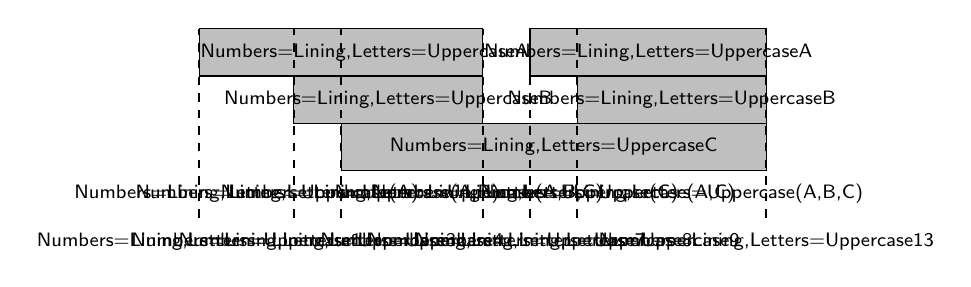
\begin{tikzpicture}[
	scale=0.6,
	every node/.append style={font=\scriptsize\sffamily\addfontfeature{Numbers=Lining,Letters=Uppercase}}]
	% boxes
	\draw [fill=lightgray] (0,4) rectangle (6,5);  % A1
	\node at (3.5,4.5) {A};
	
	\draw [fill=lightgray] (7,4) rectangle (12,5);  % A2
	\node at (9.5,4.5) {A};
	
	\draw [fill=lightgray] (2,3) rectangle (6,4);  % B1
	\node at (4,3.5) {B};
	
	\draw [fill=lightgray] (8,3) rectangle (12,4);  % B2
	\node at (10,3.5) {B};
	
	\draw [fill=lightgray] (3,2) rectangle (12,3);  % C
	\node at (7.5,2.5) {C};
	
	% item sets
	\node at (1,1.5) {(A)};
	\node at (2.5,1.5) {(A,B)};
	\node at (4.5,1.5) {(A,B,C)};
	\node at (6.5,1.5) {(C)};
	\node at (7.5,1.5) {(A,C)};
	\node at (10,1.5) {(A,B,C)};
	
	% time points
	\node at (0,0.5) {1};
	\node at (2,0.5) {3};
	\node at (3,0.5) {4};
	\node at (6,0.5) {7};
	\node at (7,0.5) {8};
	\node at (8,0.5) {9};
	\node at (12,0.5) {13};
	
	% time point lines
	\draw [dashed, thick] (0,1) -- (0,5);
	\draw [dashed, thick] (2,1) -- (2,5);
	\draw [dashed, thick] (3,1) -- (3,5);
	\draw [dashed, thick] (6,1) -- (6,5);
	\draw [dashed, thick] (7,1) -- (7,5);
	\draw [dashed, thick] (8,1) -- (8,5);
	\draw [dashed, thick] (12,1) -- (12,5);
\end{tikzpicture}
		\end{figure}
	\end{columns}
}


\section{Establishing Significance}%%%
\frame{
	\center
	{\Huge Why Significance?}
	\visible<2->{
		
		\vspace{0.2\textheight}
		
		\tikz\node[draw, rounded corners, inner sep=1em] {\LARGE qualitative \hspace{0.3\textwidth} quantitative};
	}
}
\frame{
	\frametitle{Significance -- How?}
	\begin{columns}
		\column{0.3\textwidth}
		\begin{enumerate}
			\item create 100 null distributions for every real sequence
			\item take 100 batches of 10: \\ 1 null distributions from each real distribution
			\item create distribution for every rule
			\item check real observation for significance against null observation distribution
		\end{enumerate}
		\column{0.7\textwidth}
		\only<+>{
			\begin{figure}
				\input{../aux/tikzpictures/tikz_null_naive_beamer.tex}
			\end{figure}
		}
		\only<+>{
			\begin{figure}
				\input{../aux/tikzpictures/tikz_null_naive_highlighted_beamer.tex}
			\end{figure}
		}
		\only<+>{
			\begin{figure}
				\input{../aux/tikzpictures/tikz_null_logical_beamer.tex}
			\end{figure}
		}
	\end{columns}
}

\section{Interpretation}
\frame{
	\frametitle{Interpretation}
	\begin{columns}
		\column{0.5\textwidth}
		{\color{beamerblue} Things to Keep in Mind}
		\begin{itemize}
			\item evaluate in context
			\item mothers (almost) always talk \\ ~
			\item[]~
		\end{itemize}
		\column{0.5\textwidth}
		{\color{beamerblue} Things to Look for}
		\begin{itemize}
			\item confirming existing research
			\item new ``interesting'' rules (whatever that means)
			\item generate new hypotheses
		\end{itemize}
	\end{columns}
}
\frame{
	\begin{columns}
		\column{0.5\textwidth}
		\center
		{\Huge Thank you.}
		\column{0.5\textwidth}
		{\color{beamerblue} Picture Sources}
		\begin{tabularx}{\textwidth}{>{\bfseries\tiny}r>{\tiny}X}
			lepilemur edwardsi & \copyright\ Frank Vassen \\
			callithrix jacchus & \copyright\ Raimond Spekking \\
			cebuella pygmaea & \copyright\ Don Faulkner \\
			callicebus cupreus & \copyright\ Udo Schröter \\
			saimiri & \copyright\ Ernst Vikne \\
			hylobates syndactylus & \copyright\ Su Neko\\
			orangutan & \copyright\ Trisha Shears \\
			chimpanzee & \copyright\ Frans de Waal \\
			human & \copyright\ Jelly Helm \\
		\end{tabularx}
	\end{columns}
}
\end{document}
